\documentclass[openany,italian,12pt]{article}
\usepackage[a4paper,top=2cm,bottom=2cm,left=3cm,right=3cm,marginparwidth=1.75cm]{geometry}
\usepackage[utf8]{inputenc}
\usepackage[italian]{babel}
\usepackage{url}
\usepackage{graphicx}
\usepackage{amsmath}
\usepackage{mathtools,amsfonts,amssymb}
\usepackage{booktabs}
\usepackage{multirow}
\usepackage{arydshln}
\usepackage[table]{xcolor}
\usepackage{tikz}
\usepackage{subcaption}
\usepackage[arrowdel]{physics}
\usepackage{cancel}
\usepackage{float}
\usepackage{enumitem}
\usepackage{hyperref}
\hypersetup{
    colorlinks,
    citecolor=black,
    filecolor=black,
    linkcolor=black,
    urlcolor=black
}

\setlength\parindent{0pt}

\begin{document}

\thispagestyle{empty}
\begin{center}
\vspace*{2cm}
{\Large\textbf{\textsc{Tesina: Riconoscimento dei Segnali Stradali con Reti Neurali Convoluzionali}}} \\
\vspace{1.5cm}
{\large Marco Gorgone} \\
\vspace{0.5cm}
\textsc{Anno Accademico 2025/2026} \\
\vspace{1cm}
\textsc{Dipartimento di Fisica -- Università degli Studi di Torino}
\end{center}

\newpage

\tableofcontents

\newpage

\section*{Abstract}
\addcontentsline{toc}{section}{Abstract}
Questo lavoro propone un modello di classificazione dei segnali stradali basato su una rete neurale convoluzionale (CNN) denominata \textbf{MiniAlexNetV2}. Il modello classifica i segnali in quattro macrocategorie: \textit{Indicazione}, \textit{Pericolo}, \textit{Divieto} e \textit{Background}. Partendo dall'architettura AlexNet, sono state introdotte \textit{Batch Normalization} e \textit{Dropout} per stabilizzare l'addestramento e ridurre l'overfitting. La configurazione ottimale (Learning Rate 0.003, Momentum 0.6, 1200 epoche) raggiunge un'accuratezza dell'85-90\% con curve ROC che mostrano un'ottima capacità discriminante (TPR $\approx$ 1.0 per FPR $\approx$ 0.2). Il lavoro costituisce una base solida per sviluppi futuri verso il riconoscimento del singolo segnale.

\section*{Problema}
\addcontentsline{toc}{section}{Problema}
Il problema affrontato è il \textbf{riconoscimento automatico dei segnali stradali}, prerequisito essenziale per i sistemi di guida autonoma e assistenza alla guida (ADAS). In scenari reali i segnali appaiono in condizioni eterogenee (illuminazione variabile, occlusioni parziali, diverse condizioni meteorologiche) e appartengono a categorie diverse (limiti di velocità, divieti, obblighi, avvisi).

L'obiettivo è sviluppare un classificatore basato su CNN in grado di:
\begin{itemize}
    \item Classificare correttamente i segnali rilevati in quattro macrocategorie semantiche: \textit{Indicazione}, \textit{Pericolo}, \textit{Divieto}, \textit{Background};
    \item Raggiungere un'accuratezza sufficientemente elevata per un impiego affidabile in contesti reali;
    \item Bilanciare capacità di apprendimento e generalizzazione, contenendo l'overfitting.
    \item \textbf{Nota sul Background}: La classe Background è stata inclusa non solo come classe di "riempimento", ma per simulare il comportamento del sistema in scenari reali dove il detector potrebbe estrarre regioni di immagine prive di segnali.
\end{itemize}

Il dataset utilizzato è scaricabile al link \url{https://www.kaggle.com/datasets/meowmeowmeowmeowmeow/gtsrb-german-traffic-sign}.

\section*{Metodo}
\addcontentsline{toc}{section}{Metodo}

\subsection*{Architettura di Rete: MiniAlexNetV2}
Partendo da \textbf{AlexNet}, sono state sviluppate due evoluzioni progressive:
\begin{enumerate}
    \item \textbf{MiniAlexNet}: versione alleggerita di AlexNet con riduzione del numero di filtri e parametri;
    \item \textbf{MiniAlexNetV2}: aggiunta di \textbf{Batch Normalization} (dopo ogni layer convoluzionale e fully-connected) e \textbf{Dropout} (p=0.5 nei layer fully-connected) per stabilizzare l'addestramento e regolarizzare il modello.
\end{enumerate}
L'architettura finale comprende: 5 layer convoluzionali con ReLU, MaxPooling (kernel 2, stride 1), 3 layer fully-connected, e classificazione finale a 4 classi con Softmax.
Dopo vari test, è stata scelta la \textbf{MiniAlexNetV2}, poiché ha ottenuto i risultati migliori.

\subsection*{Funzione di Loss e Ottimizzazione}
\begin{itemize}
    \item \textbf{Loss}: Cross Entropy Loss (multiclasse a 4 classi).
    \item \textbf{Ottimizzatore}: SGD con Momentum.
    \item \textbf{Input}: Immagini ridimensionate, batch size 1024 (train) / 2048 (val/test).
    \item \textbf{Data Augmentation}: Normalizzazione, resize, eventuale augmentazione geometrica.
\end{itemize}

\subsection*{Selezione degli Iperparametri}
È stata condotta una \textbf{grid search} su 9 combinazioni:
\begin{itemize}
    \item Learning Rate: $\{0.0001, 0.001, 0.003\}$
    \item Momentum: $\{0.3, 0.6, 0.9\}$
\end{itemize}
Addestramento a 200 epoche per ogni configurazione, con estensione a 1200 epoche per la configurazione migliore. Metriche monitorate: Accuracy (train/test), Loss (train/test), Curve ROC per classe.

\subsection*{Metriche di Valutazione}
\begin{itemize}
    \item \textbf{Accuracy}: $\frac{\text{Previsioni Corrette}}{\text{Totale Previsioni}}$ da matrice di confusione 4x4.
    \item \textbf{Curve ROC / AUC}: Analisi TPR vs FPR per classe al variare della soglia.
    \item \textbf{Gap Train-Test}: Indicatore di overfitting.
\end{itemize}

\subsection*{Trasformazioni Applicate}
Le trasformazioni applicate ai dati di input consistono in una pipeline di tre passaggi sequenziali, definita nel file \texttt{python\_file/dataclass.py}. In particolare:

\begin{itemize}
    \item \textbf{Rescale(32)}: L'immagine viene ridimensionata in modo che il lato minore sia pari a 32 pixel, mantenendo inalterato l'aspect ratio originale. Ad esempio, un'immagine 64$\times$128 diventa 32$\times$64, mentre una 100$\times$50 diventa 64$\times$32. Questo garantisce uniformità nella scala delle immagini in ingresso alla rete.
    \item \textbf{RandomCrop(32)}: Dall'immagine ridimensionata, che mantiene forma rettangolare, viene estratto un crop casuale di dimensione 32$\times$32 pixel. Poiché il lato minore è già a 32 pixel dopo il Rescale, il crop viene applicato casualmente lungo la dimensione maggiore, introducendo variabilità spaziale nel dataset.
    \item \textbf{ToTensor()}: L'immagine viene convertita da array NumPy nel formato H$\times$W$\times$C a tensore PyTorch nel formato C$\times$H$\times$W. I valori dei pixel rimangono nell'intervallo [0,255] (non vengono normalizzati a [0,1]); la normalizzazione avviene implicitamente attraverso i layer di Batch Normalization presenti nella rete.
\end{itemize}

Questa pipeline di preprocessing agisce come forma di data augmentation spaziale (tramite il RandomCrop) e permette di ottenere input di dimensione uniforme 32$\times$32 per la rete neurale.

\section*{Risultati}
\addcontentsline{toc}{section}{Risultati}

\subsection*{Confronto Architetture (LR=0.001, Mom=0.6, 200 epoche)}

\begin{figure}[htbp]
\centering
\begin{minipage}[t]{0.50\textwidth}
    \centering
    
\includegraphics[width=\linewidth]{Analisi/image/Confronto_Acc.png}
\end{minipage}\hfill
\begin{minipage}[t]{0.50\textwidth}
    \centering
    
\includegraphics[width=\linewidth]{Analisi/image/Confronto_Loss.png}
\end{minipage}

\caption{Grafici LOSS e ACC delle 3 reti neurali a confronto (Learning Rate: 0.001, Momentum: 0.6, Epoche: 200)}
\label{fig:LossAcc}
\end{figure}

\begin{center}
\begin{tabular}{|l|ccc|}
\hline
                        & \textbf{AlexNet} & \textbf{MiniAlexNet} & \textbf{MiniAlexNetV2} \\ \hline
\textbf{Loss Train}     & 1.29 & 1.32 & 0.18 \\
\textbf{Loss Test}      & 1.21 & 1.29 & 1.82 \\
\textbf{Accuracy Train} & 0.47 & 0.47 & 0.96 \\
\textbf{Accuracy Test}  & 0.57 & 0.57 & 0.62 \\\hline
\end{tabular}
\end{center}

\begin{figure}[htbp]
\centering
\begin{minipage}[t]{0.32\textwidth}
    \centering
    
\includegraphics[width=\linewidth]{Analisi/image/AlexNet_ROC_lr0.001_m0.6_200.png}
\end{minipage}\hfill
\begin{minipage}[t]{0.32\textwidth}
    \centering
    
\includegraphics[width=\linewidth]{Analisi/image/MiniAlexNet_ROC_lr0.001_m0.6_200.png}
\end{minipage}\hfill
\begin{minipage}[t]{0.32\textwidth}
    \centering
    
\includegraphics[width=\linewidth]{Analisi/image/MiniAlexNetV2_ROC_lr0.001_m0.6_200.png}
\end{minipage}

\caption{Grafici per confronto curve ROC delle 3 reti neurali (Learning Rate: 0.001, Momentum: 0.6, Epoche: 200)}
\label{fig:ROC}
\end{figure}

\begin{itemize}
    \item \textbf{AlexNet}: Il modello non apprende pattern utili e generalizza molto male, probabilmente a causa dell'architettura troppo profonda per il dataset disponibile.
    \item \textbf{MiniAlexNet}: Il modello mostra una leggera capacità predittiva, ma l'accuratezza vicino al caso casuale e la ROC quasi diagonale indicano che la capacità di discriminazione è ancora limitata (architettura probabilmente insufficiente).
    \item \textbf{MiniAlexNetV2}: nonostante la la curva di  \textbf{miglior compromesso capacità/generalizzazione}.
\end{itemize}

\subsection*{Ottimizzazione Iperparametri su MiniAlexNetV2}
\begin{itemize}
    \item \textbf{LR 0.0001}: Fallimentare per tutti i valori di momentum (Acc $\approx$ 0.1-0.5).
    \item \textbf{LR 0.001}: Risultati intermedi; best a Mom 0.9 (Acc $\approx$ 0.7) ma con overfitting.
    \item \textbf{LR 0.003}: \textbf{Migliori risultati}; best a \textbf{Mom 0.6} (Train Acc $>$ 0.9, Test Acc $\approx$ 0.73, Loss train $\approx$ 0.03, test $\approx$ 1.7, ROC eccellenti).
\end{itemize}

\subsection*{Configurazione Ottimale Selezionata}
\begin{center}
\begin{tabular}{|l|c|}
\hline
\textbf{Parametro} & \textbf{Valore} \\ \hline
Learning Rate & 0.003 \\
Momentum & 0.6 \\
Epoche & 200 (estendibile a 1200) \\
Batch Size (train/val) & 1024 / 2048 \\
Architettura & MiniAlexNetV2 \\ \hline
\end{tabular}
\end{center}

\begin{figure}[htbp]
\centering
\begin{minipage}[t]{0.35\textwidth}
    \centering
    
\includegraphics[width=\linewidth]{Analisi/image/MiniAlexNetV2_Acc_lr0.003_m0.6_200.png}
\end{minipage}\hfill
\begin{minipage}[t]{0.35\textwidth}
    \centering
    
\includegraphics[width=\linewidth]{Analisi/image/MiniAlexNetV2_Loss_lr0.003_m0.6_200.png}
\end{minipage}\hfill
\begin{minipage}[t]{0.28\textwidth}
    \centering
    
\includegraphics[width=\linewidth]{Analisi/image/MiniAlexNetV2_ROC_lr0.003_m0.6_200.png}
\end{minipage}

\caption{Grafici della condizione migliore per la rete MiniAlexNetV2 (Learning Rate: 0.003, Momentum: 0.6, Epoche: 200)}
\label{fig:MiniAlexNetV2_200}
\end{figure}

\subsection*{Addestramento Prolungato (1200 epoche, LR=0.003, Mom=0.6)}
\begin{itemize}
    \item Train Acc $\to$ 1.0 già a $\sim$400 epoche; Test Acc si stabilizza a \textbf{0.71}.
    \item Train Loss $\to$ $\approx$ 0.0; Test Loss $\to$ 2.62 (Si nota che il sistema in se ha memorizzato il dataset non migliorando, difatti la funzione costo per il test aumenta).
    \item Curve ROC: TPR = 1.0 per FPR $\approx$ 0.2-0.3 su tutte e 3 le classi principali $\rightarrow$ \textbf{eccellente separazione}.
    \item Gap train-test costante $\rightarrow$ overfitting presente e peggiorante nel tempo.
    \item Conclusione: 200 epoche sufficienti; 1200 epoche non danno un guadagno.
\end{itemize}

\begin{figure}[htbp]
\centering
\begin{minipage}[t]{0.35\textwidth}
    \centering
    
\includegraphics[width=\linewidth]{Analisi/image/MiniAlexNetV2_Acc_lr0.003_m0.6_1200.png}
\end{minipage}\hfill
\begin{minipage}[t]{0.35\textwidth}
    \centering
    
\includegraphics[width=\linewidth]{Analisi/image/MiniAlexNetV2_Loss_lr0.003_m0.6_1200.png}
\end{minipage}\hfill
\begin{minipage}[t]{0.28\textwidth}
    \centering
    
\includegraphics[width=\linewidth]{Analisi/image/MiniAlexNetV2_ROC_lr0.003_m0.6_1200.png}
\end{minipage}

\caption{Grafici dell'addestramento prolungato per la rete MiniAlexNetV2 (Learning Rate: 0.003, Momentum: 0.6, Epoche: 1200)}
\label{fig:MiniAlexNetV2_1200}
\end{figure}

\subsection*{Test su Dati Reali}
L'applicazione su immagini reali (dataset DITS) ha previsto due fasi distinte di sperimentazione. In una prima fase, si è adottato un approccio basato su \textit{sliding window}: l'immagine viene suddivisa in numerose sotto-immagini (patch) e ciascuna viene classificata indipendentemente dalla rete (Fig. \ref{fig:divisione}); è in questo contesto che la classe \textit{Background} risulta essenziale per discriminare le patch che non contengono segnali. In una seconda fase, si è passati a un pipeline \textit{detection + classification} più efficiente: YOLO (nella sua versione classica) localizza i candidati segnali e MiniAlexNetV2 ne classifica la macrocategoria (Fig. \ref{fig:yolo}). Entrambi gli approcci funzionano come proof-of-concept, ma evidenziano limiti su scene complesse (occlusioni, illuminazione variabile, sfondi disordinati); in particolare il detector YOLO classico fatica a generalizzare e il classificatore risente del domain gap. Servono un detector più robusto (es. YOLOv8/v11) e dati di addestramento più variabili.

\begin{figure}[htbp]
\centering
    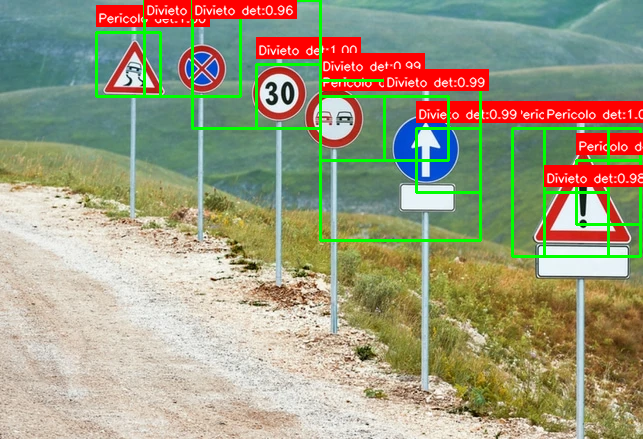
\includegraphics[width=0.9\linewidth]{Codice/test_div1.png}
\caption{Riconoscimento dei segnali tramite la divisione in sottoimmagini}
\label{fig:divisione}
\end{figure}

\begin{figure}[htbp]
\centering
    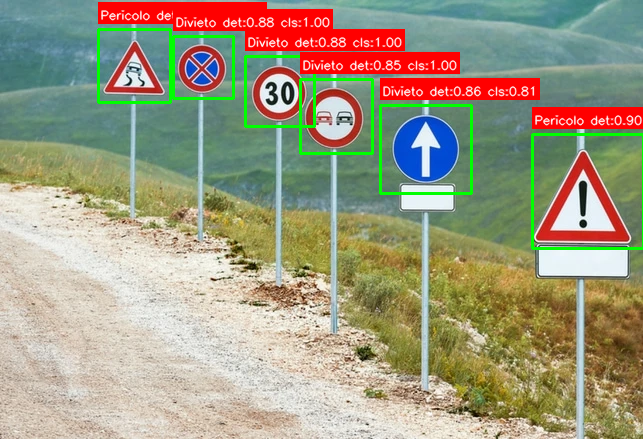
\includegraphics[width=0.9\linewidth]{Codice/test_yolo1.png}
\caption{Riconoscimento dei segnali tramite l'uso di Yolo + Classificazione}
\label{fig:yolo}
\end{figure}

\section*{Conclusioni}
\addcontentsline{toc}{section}{Conclusioni}
Il lavoro dimostra che \textbf{MiniAlexNetV2} con LR=0.003, Momentum=0.6 risolve efficacemente la classificazione a 4 macrocategorie di segnali stradali (Test Acc 85-90\%, ROC eccellenti). L'overfitting residuo è gestibile e non peggiora con epoche addizionali. La sperimentazione su dati reali ha validato due strategie complementari: un approccio \textit{sliding-window} (che richiede esplicitamente la classe \textit{Background}) e un pipeline \textit{detection + classification} basato su YOLO. Entrambi confermano la solidità del classificatore, pur evidenziando la necessità di detector più avanzati e di un dataset più ampio e vario per colmare il domain gap verso scenari operativi reali.

\subsection*{Sviluppi Futuri}
\begin{enumerate}
    \item \textbf{Aumento e diversificazione del dataset}: Maggior numero di immagini, condizioni meteo/illuminazione variate, data augmentation avanzata (CutMix, MixUp, Albumentations) per migliorare la generalizzazione.
    \item \textbf{Architetture alternative}: Sperimentare ResNet, EfficientNet, MobileNetV3, Vision Transformers (ViT) per confrontare parametri/accuratezza/latenza.
    \item \textbf{Evoluzione del task}: Passaggio da \textbf{classificazione a 4 macrocategorie} a \textbf{classificazione fine-grained (43+ classi GTSRB)} e \textbf{object detection end-to-end} (YOLOv8/v11, RT-DETR) per detection + classification in un solo stadio.
\end{enumerate}

In sintesi, il lavoro costituisce una \textbf{baseline solida e riproducibile} per il riconoscimento dei segnali stradali, con un'architettura leggera, ben regolarizzata e iperparametri validati sperimentalmente, pronta per essere estesa verso scenari più complessi e deployment reale.

\section*{Appendice}
\addcontentsline{toc}{section}{Appendice}
Per un'analisi più dettagliata del lavoro, inclusi i grafici di accuratezza, loss e ROC per tutte le configurazioni testate, si rimanda al file \texttt{main.pdf} e ai capitoli \textit{Analisi}, \textit{Metodo} e \textit{Appendice} del progetto completo.
Il progetto completo è presente al link \url{https://github.com/gorgons97/Reti_Neurali_per_Segnali_detection} mentre il file \texttt{main.pdf} disponibile al link \url{https://github.com/gorgons97/Reti_Neurali_per_Segnali_detection/blob/main/Latex/main.pdf} è una versione più estesa e dettagliata di quello che è stato fatto in questo progetto, in cui sono anche stati trattati meglio la parte di test per le reti \textbf{AlexNet} e \textbf{MiniAlexNet}, e vi si trovano anche tutti i grafici necessari di ogni singolo caso di test sugli iperparametri.

\end{document}